\subsection{Extensible Data Acquisition Tool} \label{background:svein}
In the thesis "Extensible data acquisition tool for Android" by Gjøby \cite{gjoby} a proposition of a \textit{data acquisition system} for Android is presented. The thesis proposes a system that hides the low-level sensor-specific details into two components, \textit{providers} and \textit{sensor wrappers}. The provider is responsible for the functionality that is common for all data sources (e.g., starting and stopping the data acquisition), while the sensor wrapper is responsible for the data source specific functionality (e.g., communicating with the data source).

The thesis solves the difficulties around creating an extensible data acquisition tool, connecting new and existing sensors, and finding a common interface. The problem statement of the thesis addresses the following concerns regarding sensors:
\begin{itemize}
    \item \textit{Common abstraction/interface for the interchanged data}\\ 
    Sensor platform manufacturers have their low-level protocol to support the functionality of their product. Typically, the manufacturers provide software development kits (SDKs) to hide the low-level protocols so third-party developers can be easier; however, both the low-level protocol and the SDKs are not standardized. Thus, for each sensor, there might be different commands and methods.
    \item \textit{Various Link Layer technologies} \\ 
    Each sensor might use different Link Layer technology (i.e., Ethernet, USB, BlueTooth, WiFi, ANT+, and ZigBee), which means establishing a connection between a device and a sensor might differ. For instance, BlueTooth devices need to be paired, while devices on the WiFi can address each other without any pairing. 
    \item \textit{Reusability of sensor code}\\
    Applications that implement support for the low-level protocol of a sensor type can not be shared between different applications. Thus, introducing duplicate work and code if multiple application wish to use the same sensor type. A framework that isolates the sensor that applications can use, might make it easier for application to utilize the collected data. In addition, isolating the sensors into modules improves the robustness and quality of the implementation. 
    
\end{itemize}

In the thesis, the goal is to develop an extensible system, which enables applications to collect data from various external and built-in sensors through one common interface. The solution around an extensible system is to have the core of the application unchangeable when adding support for a new data source, regardless of the Link Layer technology and communication protocol used by the data source. Making all the data sources behave as the same, is a naive solution to the problem. However, separating the software into two different components, a \textit{provider} component and a \textit{sensor wrapper} component, enables the reuse of functionality that is common amongst the data sources. 

The sensor wrapper application is tailored to suit the Link Layer technology and data exchange protocol of one particular data source. Additionally, responsible for connectivity and communication with the data source. The provider application is responsible for managing the sensor wrappers---starting and stopping the data acquisition---and processing the data received from the sensor wrapper application. Thus, everything that is independents of the data source should be a part of the provider application. With this type of solution, the possibility to reuse the sensor wrapper application for different provider applications is made possible. However, there are some overheads with this solution. Mostly, the inter-process communication that might be costly and increase the complexity of the code. Nonetheless, the flexibility and extensibility gained by separating the functionalists out weights the cost.

When a connection is established with the provider application, a package of metrics and data type (all the data does not change during the acquisition as metadata) is sent describing the context of the data collected. The metadata is necessary because different sensors might sample data in different environments, and some applications are depending on recognizing the environment of the data acquisition. Therefore, it is critical to know what data values are measured. Consequently, exposing sensors and data channels through one common interface requires a field of metadata which can be used to: (1) \textit{distinguish} sensor wrapper and data channel the data originated from; (2) determine the \textit{capabilities} of the sensors (i.e., EEG, ECG, LUX); (3) determine the \textit{unit} the data is represented in (i.e., for temperature, Celsius or Fahrenheit); (4) describing the data channel (i.e., placement of the sensor); and (5) a timestamp of when the data was sampled. 

To summarize, the task of a \textit{sensor wrapper} is to establish a connection to and collect data from precisely one specified data source, and to send the collected data to the \textit{provider application} that is listening for it. A data source (e.g., BiTalion) can have support for multiple sensor attachments (defined as data channel in the thesis), although, only on sensor wrapper is necessary for each data source and their data channels. Each sensor wrapper is tailored to adapt to the data source's Link Layer technology and the communication protocol of a respective data source. Upon activation by a provider application, the data is collected by the sensor wrapper, and pushed to the provider application in a JSON-format. An illustration of the structure is found in Figure \ref{fig:provider_SW}.

\begin{figure}
    \centering
    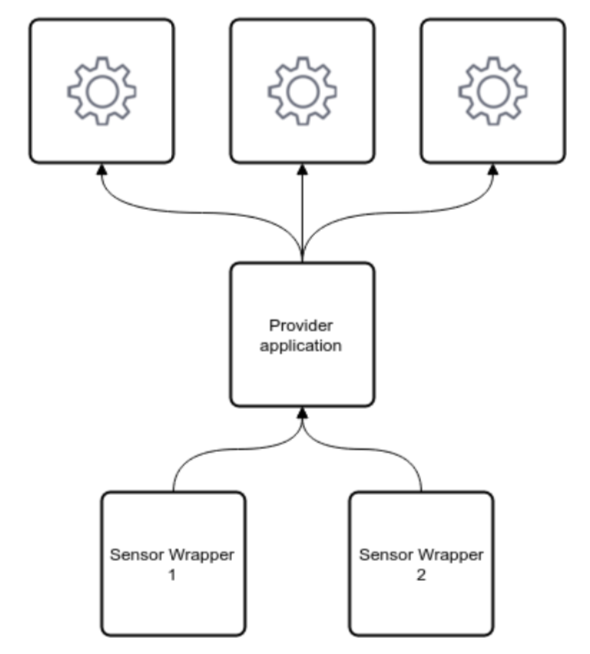
\includegraphics[width=0.5\textwidth]{images/provider_SW.png}
    \caption{Sharing the collected data between multiple applications \cite{gjoby}}
    \label{fig:provider_SW}
\end{figure}